\documentclass{article}

\usepackage{graphicx}

\author{Nic Hollingum - 308193415}
\title{Computer and Network Security - Assignment 1}

\addtolength{\oddsidemargin}{-.5in}
\addtolength{\evensidemargin}{-.5in}
\addtolength{\textwidth}{1in}
\addtolength{\topmargin}{-0.5in}
\addtolength{\textheight}{1.5in}

\begin{document}
\maketitle

\section{DES}
\subsection{DESV}
First we note the dependancy between $k$ and $k_1$.
If we are able to break $k$ we are immediately able to break $k_1$ by xoring a single plain/cipher pair with the encryption of only $k$:

$(DES_k (m) \oplus 0) \oplus (DES_k (m) \oplus k_1) = 0 \oplus k_1 = k_1$

In order to find $k$ we need to perform the DES cracking by somehow removing $k_1$ from the problem.
Again we require only a few plain/cipher pairs (2).
We Note that be xoring the ciphertext we can strip $k_1$ from the output:

$(DES_k (m_1) \oplus k_1) \oplus (DES_k (m_2) \oplus k_1) = DES_k (m_1) \oplus DES_k (m_2)$

Then we simply find the $k$ for which this holds.
This requires strictly twice the number of encryptions/decryptions to normally brute force DES, since we must encrypt 2 messages each check.
On average this means $O(2^{56})$ enc/decyyptions for a key of length 56, as indeed $k$ is.
More intelligent attaks can reduce this figure.

\subsection{DESW}
Breaking this ``enhanced'' DES requires little more effort than regular DES.
First we note that if we had $k$ we can instantly gain $k_1$ by decrypting one of our ciphertexts and xoring that with its plain pair.
However this has to be true for all of our plain/cipher pairs, so we know something about $k_1$ even without knowing $k$.
Namely, when we decrypt pair i or j with k: $DES_k (c_i) \ne m_i$ but, $DES_k (c_i) \oplus DES_k(c_j) = m_i \oplus m_j$.
Or more intuitively, when we have the right $k$, every plaintext pair will be just as different from the decryption as each other.

Thus we have our algorithm for breaking DESW.
We brue force $k$, and compare the difference between the decryption of one ciphertext and the decryption of another.
If the 2 differences are not the same, then $k$ was not chosen correctly, and we continue.
Otherwise, we have chosen the correct $k$.
Now $k_1$ is easily retrieved: $DES_k (c_i) \oplus m_i = k_1$.

\section{Hash Functions}

\subsection{Ciphers using Hash Functions}

\begin{figure}[htb]
\begin{center}
\leavevmode
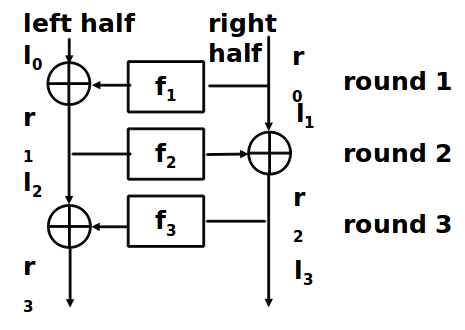
\includegraphics[width=0.4\textwidth]{feistel.png}
\end{center}
\label{fig:vortrap}
\end{figure}

This is a Feistel network, as discussed in lectures/textbooks.
This particular image was taken from Lecture slides.
This network can be used to create block ciphers using normally non-reversible functions, in our case hash functions.

We are able to decrypt this normally one-way function because we never fully hashed the input, only half at a time (for each block).
We are able to use the most recently un-hashed half in order to work out what the result would have been, the net effect is to peel off a single layer of hashing from the block, at which point we can do the same for the blocks reversed, and so on until we have the original block.

\subsection{Ciphers as Hash Functions}

Here we see an aplication of the birthday attack.
Naively we can point out that the birthday bound (accoring to Wikipedia) for an n bit hash can be approximated by $\sqrt{{\pi \over 2}2^n}$.
This tells us the expected number of inputs we would have to brute force in order to have a 50\% chance of a collision, i.e. by which time we would expect to have at least 1.
For a 64 bit hash (like md5, and the DES-hash from this question) this means roughly 5.3 billion messages, a significant improvement on the  18 quintillion ($1.8 \times 10^{19}$) message space.

However, given the nature of the hash we can improve this bound slightly.
Given 2 messages $m_1$ and $m_2$ which hash to the same digest $d$, we see that $m_1 + m_x$ and $m_2 + m_x$ also collide with the same digest $d_x$ for some message $m_x$.
This is because the hash function is simply performing DES using the same key (the blocks of $m_x$) on the same input ($d$).
This also works in reverse, i.e. we can exclude messages which end with identical blocks if their non-identical starts didn't collide.
A similar principal allows us to combine colliding hashes into colliding hash-groups.
So if $m_1$ and $m_2$ collide, and $m_3$ and $m_4$ collide, then $m_1 + m_3$ and $m_2 + m_4$ will also collide, as will $m_1 + m_4$ and $m_2 + m_3$.

We use this observation to limit out choices of $m_1$ and $m_2$.
From above: the messages must be a different number of blocks, and from the nature of DES: any 2 block message must collide with 1 1 block message.
Therefore we arbitrarily choose some initial block for $m_2$ (call it $m_a$) and begin brute force searching its 2nd block and the 1st block of $m_1$.
Then we are now looking for 2 keys $k_1$ and $k_2$ such that $DES_{k_1}(IV) = DES^{-1}_{k_2}(DES_{m_a}(IV))$.
Since DES only has a search sapce of $2^{56}$ bits, and we require 2 such keys (so twice that) this can be done in approximately $\sqrt{{\pi \over 2}2^{57}}$ iterations, or under 1/2 a billion tries.

\subsection{Ciphers as Hash Functions 2}

This task is normally considered much harder than the above.
The birthday paradox specified that only some 2 of the set had to collide, and in a set of size n we had $n \choose 2$ possible colliding pairs.
However now we only have $n$ possible colliding pairs (since the pair must contain d), and our required search space will be ${n \choose 2} \over {n}$ times larger.
In fact it will roughly equate to brute force on the entire search space.

However this is not a normal hash function.
It is impossible to work backwards to find the m that generated some d, since each block of m will generate a new d to be fed into DES for the next block's key.
Therefore if we find any key (which corresponds to m) that allows us to go backwards to the stage before m, we have no idea whether this $m'$ is meant to be the IV, or some block which needs to be reversed again.
But finding any message $m_x$ which hashes to our digest means we only need to greedily seek the IV and remember our key choices along the way.
Therefore this problem reduces to a known plaintext attack on DES, where we try to find the key which will decrypt our ciphertext d to the plaintext IV.
This is known to be doable in $O(2^55)$ iterations on average, which is again significantly better than brute force on the message space ($3.6 \times 10^{16}$ vs $1.8 \times 10^{19}$).
 
\section{Protocol Analysis}

For authentication this protocol has 2 key features.
Firstly no secret information is leaked (and therefore we can say no one is able to impersonate the one who made v and n).
Secondly this protocol contains challenge response, which makes it difficult for someone to pretend to be Alice when chalanged by another.
We use the notation ${a_b}$ to denote a modulo b.

First we note that it is impossible to determine r from ${r^2}_n$ given sufficiently large choice of r.
Therefore after an authentication step, Bob will only know the $r_n$ for those ${r^2}_n$ in subset 2, and cannot know those from subset 1.
It is also impossible to work out s from ${sr}_n$, given that details of s are hidden behind the $r_n$ which we noted above could not be worked out.
Nor is it possible to contrive some r and x for which ${({xr}_n)^2}_n = {vr^2}_n$.
This is how we can say that only the one who knows the secret s, which nobody else can work out, is able to perform authentication.

The other important point of this protocol is the challenge/response.
There would be problems if Bob were not given some task to make Alice prove her identity, namely bob could replay the procedure to anyone else and so pretend to be Alice himself.
Forcing the authenticating party to perform this action multiplies the work required by an imposter.
For alice to authenticate herself, she only needs to know s, and she can make ${sr}_n$ for any r she happens to randomly generate.
She can also prove that it was her who randomly generated that r by providing it modulo n to compare with the ${r^2}_n$ she sent earlier.
The down side is that a potential imposter is able to provide an ${sr}_n$ for given ${r^2}_n$ if the party they are pretending to authenticate to places that $r^2$ in subset 1.
Similarly the potential imposter can provide the $r_n$ for and ${r^2}_n$ placed in subset 2.
In this way if an attacker sees ${r^2}_n$ more than once, this would allow them to authenticate with this r to anyone else.
For this reason first a sufficiently large k (maybe 1024) should be chosen to make acquiring this many pairs difficult, but second a sufficiently large r space must be chosen as well.
By the birthday paradox if alice chooses k r's randomly for each authentication, and we require k pairs of the same number chosen twice, then we would have to sit through approximately ${k 2^{|r| \over 2}} \over {k}$ authentication procedures.

Therefore these 2 mechanisms mean that Alice is able to authenticate as the one who holds s where only Alice can answer questions about s (subset 1), only the one who generated r can prove it (subset 2) and nobody can reasonably gain enough information to authenticate as Alice.

\section{Protocol Design}

\subsection*{A}
The protocol is trivially secure, in that Bob has no way of knowing what x was committed before Alice opens.
Alice is choosing some r and xoring that with x, then sending the xored output to Bob.
This is essentially a 1-time pad, r is truly random and therefore the output y looks truly random, and there is no way for bob to know what was xored with what until Alice tells him.

\subsection*{B}
This protocol is trivially not binding, in that Alice can reveal a value she did not commit.
We show that no matter what bits Alice sends Bob, she can calim that r was any arbitrary value in order to show bob that x was any arbitrary value, even after she has sent y, the supposed xor of r and x.

Let us suppose that alice sends y which really was $x \oplus r$ for random r and a good guess x.
But now alice wishes to say that she in fact guessed $x'$, this is trivially easy since $y = x \oplus r$ then we simply pretend we chose $r'$ such that $y = x' \oplus r'$.
Or more formally:

$x \oplus r = x' \oplus r'$

$x \oplus r \oplus x' = r'$

Then Alice simply sends $r'$ instead of r and Bob will think alice initially committed $x'$ instead of x.

\subsection*{C}

The reality is, xoring, by virtue of being fully reversible, cannot simultaneously provide security and bindingness.
We shall use Hash functions to provide security, and nonces to provide freshness.

\begin{itemize}
	\item Bob sends Alice $n_b$, a nonce of some decent length (256 bits, we shall say)
	\item Alice formulates her own nonce $n_a$ of the same length
	\item Alice sends Bob $H(n_a + n_b + x)$ or the hash of a message made by appending bob's nonce to alice's, and the x value to that.
	\item {\bf Commit:} Alice sends bob $n_a$ and x, Bob verifies that Alice indded gave him $H(n_a + n_b + x)$ originally
\end{itemize}

This mechanism, though more complicated, provides both security and bindingness.
Alice's nonce $n_a$ is used to ensure bob is unable to brue-force the message space in advance.
If it were not there (and the message to be hased was, say $n_b + x$) then Bob could precompute all messages of the form $n_b + c$ then determine x before alice has committed.
Its presence means that $2^{|n_a|}$ different messages could be the origin of the same x, and thus x is reasonably unknowable.
This works similarly in reverse for Bob's nonce, in that alice cannot pre-compute messages grant her a different x, Alice would also have to precompute such collisiions which also have the $n_b$ nonce after hers, for any nonce Bob could provide.
Alice is therefore unable to work out in advance some colliding messages, and therefore cannot dupe the system.
We presume that a sufficiently good hash (sha256 for example) was chosen to prevent alice from attempting to brute force collisions after receiving Bob's nonce and before comitting.

\end{document}
